\documentclass[border=2pt]{standalone}
\usepackage{tikz}
\usepackage{pgfplots}
\begin{document}
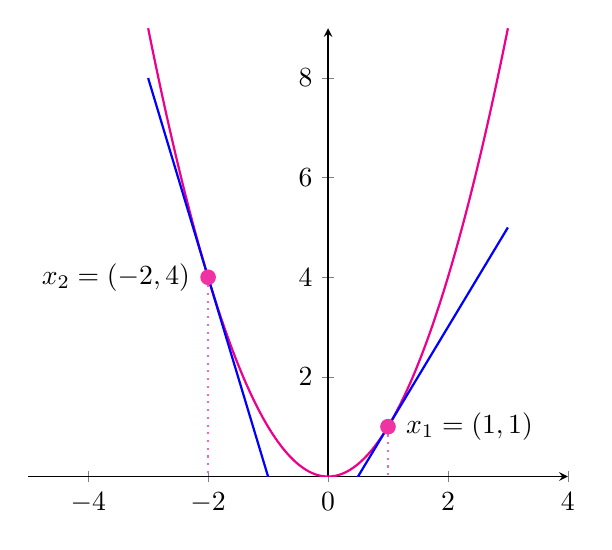
\begin{tikzpicture}
    \begin{axis}[%
        %,xlabel=$Q$
        %,ylabel=$P$
        ,xmin=-5,xmax=4
        ,ymin=0,ymax=9
        ,axis x line=bottom
        ,axis y line=middle
        ,every axis x label/.style={at={(current axis.right of origin)},anchor=west}
        ,every axis y label/.style={at={(current axis.north west)},anchor=south}
        ]
    \addplot[%
        ,samples=1024,domain=-3:3
        ,smooth
        ,thick
        ,magenta
        ] {(x*x)};

    \addplot[domain=0:3, thick, blue]{2*x - 1};
    \addplot[domain=-3:0, thick, blue]{-4*x - 4};

    \addplot[dotted, thick, magenta!60] coordinates {(1,1) (1,0)};
    \addplot[dotted, thick, magenta!60] coordinates {(-2,4) (-2,0)};

    \node[label={0:{$x_1=(1,1)$}},circle,fill=magenta!80,inner sep=2pt] at (axis cs:1,1) {};
    \node[label={180:{$x_2=(-2,4)$}},circle,fill=magenta!80,inner sep=2pt] at (axis cs:-2,4) {};

    \end{axis}

\end{tikzpicture}
\end{document}
